\documentclass[tikz,border=8pt]{standalone}
\usepackage{amsmath}
\usetikzlibrary{arrows.meta,positioning,calc,shapes.geometric,fit,backgrounds}

\definecolor{shapcolor}{RGB}{255,215,0}   % yellow
\definecolor{ffacolor}{RGB}{34,139,34}    % green
\definecolor{consensuspurple}{RGB}{128,90,180}
\definecolor{softgray}{RGB}{245,245,245}
\definecolor{linegray}{RGB}{60,60,60}

\tikzset{
  flow/.style={-Latex, very thick, draw=linegray},
  poolbox/.style={
    draw=linegray, thick, rounded corners=2pt,
    fill=softgray, align=left,
    minimum width=4.0cm, minimum height=3.8cm,
    inner sep=8pt
  },
  procbox/.style={
    draw=linegray, thick, rounded corners=2pt,
    fill=white, align=center,
    minimum width=2.8cm, minimum height=1.0cm
  },
  decision/.style={
    diamond, draw=linegray, thick, fill=white,
    aspect=1.5, align=center, inner sep=1.5pt,
    minimum width=2.2cm, minimum height=1.3cm
  },
  outbox/.style={
    draw=linegray, thick, rounded corners=2pt,
    fill=white, align=center,
    minimum width=3.2cm, minimum height=1.1cm
  },
  note/.style={
    align=left, font=\small, text width=15.5cm
  }
}

\begin{document}
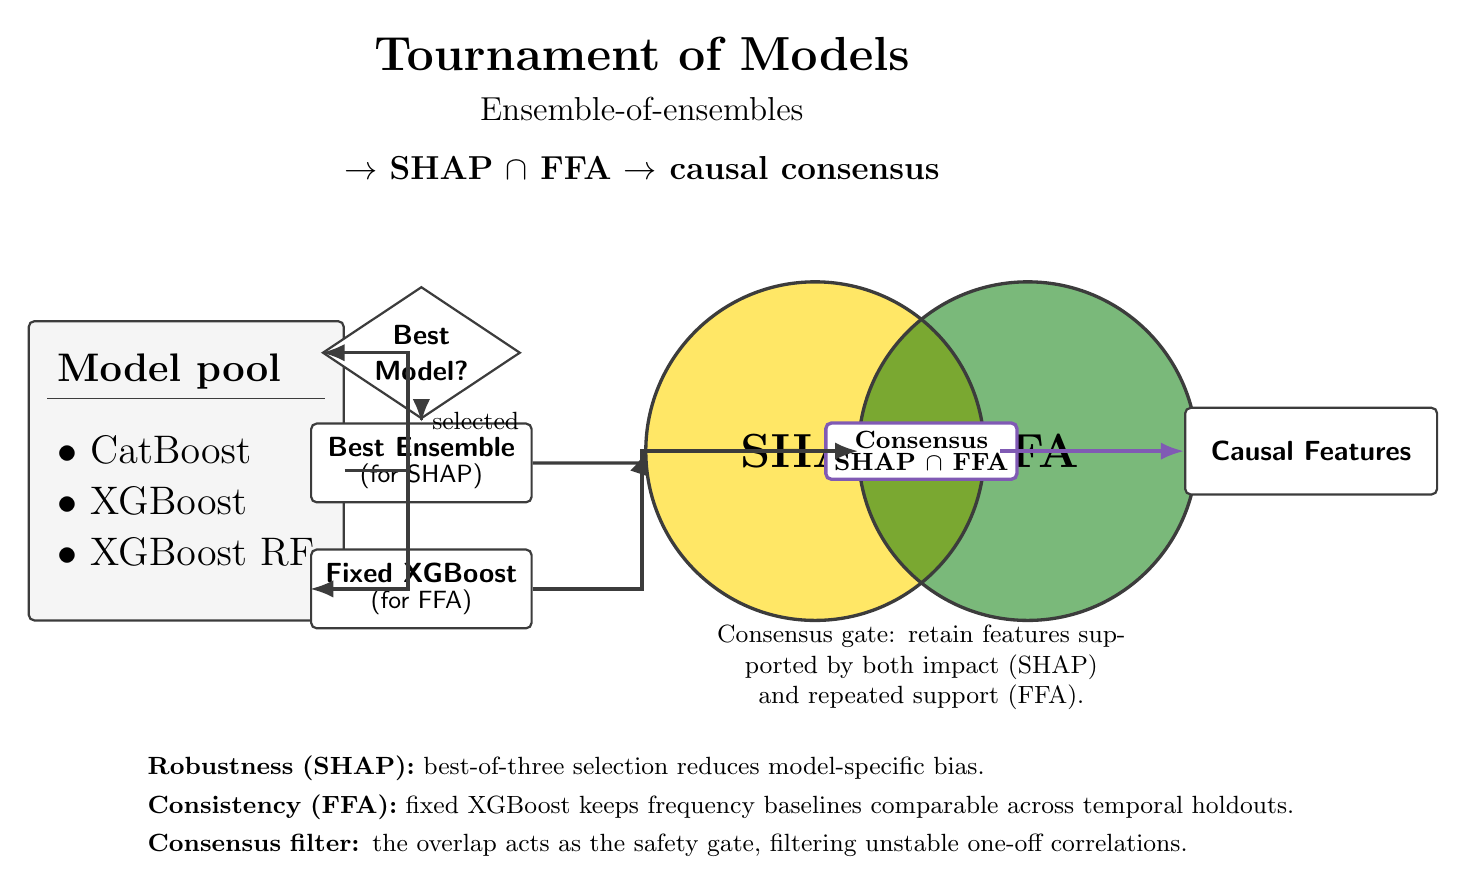
\begin{tikzpicture}[font=\sffamily]

%--------------------------------------------------
% Title block
%--------------------------------------------------
\node[font=\bfseries\LARGE, align=center] (title) at (8.0,8.8)
{Tournament of Models};

\node[font=\large, align=center] at (8.0,8.1)
{Ensemble-of-ensembles};

\node[font=\bfseries\large, align=center] at (8.0,7.35)
{$\rightarrow$ SHAP $\cap$ FFA $\rightarrow$ causal consensus};

%--------------------------------------------------
% Left: model pool
%--------------------------------------------------
\node[poolbox, anchor=west] (pool) at (0.2,3.5) {};

\node[anchor=north west, font=\bfseries\Large] at ([xshift=0.25cm,yshift=-0.3cm]pool.north west)
{Model pool};

\draw[linegray, thin] ([xshift=0.25cm,yshift=-1.0cm]pool.north west) --
                      ([xshift=-0.25cm,yshift=-1.0cm]pool.north east);

\node[anchor=north west, font=\Large] at ([xshift=0.25cm,yshift=-1.35cm]pool.north west)
{$\bullet$ CatBoost};

\node[anchor=north west, font=\Large] at ([xshift=0.25cm,yshift=-2.0cm]pool.north west)
{$\bullet$ XGBoost};

\node[anchor=north west, font=\Large] at ([xshift=0.25cm,yshift=-2.65cm]pool.north west)
{$\bullet$ XGBoost RF};

%--------------------------------------------------
% Decision and branch boxes
%--------------------------------------------------
\node[decision] (bestq) at (5.2,5.0) {\textbf{Best}\\[1pt]\textbf{Model?}};

\node[procbox] (bestens) at (5.2,3.6) {\textbf{Best Ensemble}\\[-1mm]\small(for SHAP)};

\node[procbox] (fixedxgb) at (5.2,2.0) {\textbf{Fixed XGBoost}\\[-1mm]\small(for FFA)};

% arrows from pool to decision / fixed path
\draw[flow] (pool.east) -- ++(0.8,0) |- (bestq.west);
\draw[flow] (pool.east) -- ++(0.8,0) |- (fixedxgb.west);

\draw[flow] (bestq.south) -- node[right, font=\small] {selected} (bestens.north);

%--------------------------------------------------
% SHAP / FFA circles
%--------------------------------------------------
\coordinate (shapc) at (10.2,3.75);
\coordinate (ffac)  at (12.9,3.75);

% filled circles with strong intersection
\begin{scope}[blend mode=multiply]
  \fill[shapcolor, opacity=0.60] (shapc) circle (2.15cm);
  \fill[ffacolor, opacity=0.60]  (ffac)  circle (2.15cm);
\end{scope}

\draw[linegray, very thick] (shapc) circle (2.15cm);
\draw[linegray, very thick] (ffac)  circle (2.15cm);

\node[font=\bfseries\LARGE] at (shapc) {SHAP};
\node[font=\bfseries\LARGE] at (ffac)  {FFA};

% intersection label
\node[
  draw=consensuspurple,
  very thick,
  rounded corners=2pt,
  fill=white,
  inner sep=3pt,
  font=\bfseries\small,
  align=center
] (consensuslabel) at ($(shapc)!0.5!(ffac)$)
{Consensus\\[-1mm]\small SHAP $\cap$ FFA};

%--------------------------------------------------
% Branch arrows to circles
%--------------------------------------------------
\draw[flow] (bestens.east) -- (8.0,3.6) -- ([xshift=-2.15cm]shapc);

\draw[flow] (fixedxgb.east) -- (8.0,2.0) |- ([xshift=-2.15cm]ffac);

%--------------------------------------------------
% Output: Causal Features to the right
%--------------------------------------------------
\node[outbox] (causal) at (16.5,3.75) {\textbf{Causal Features}};

% arrow from overlap region to output
\draw[flow, consensuspurple] ($(shapc)!0.5!(ffac)+(1.0,0)$) -- (causal.west);

%--------------------------------------------------
% Optional small caption under circles
%--------------------------------------------------
\node[font=\small, align=center, text width=6cm] at (11.55,1.0)
{Consensus gate: retain features supported by both impact (SHAP) and repeated support (FFA).};

%--------------------------------------------------
% Compact explanatory notes
%--------------------------------------------------
\node[note, anchor=north west] (notes) at (1.6,0.0) {
\textbf{Robustness (SHAP):} best-of-three selection reduces model-specific bias.\\[1mm]
\textbf{Consistency (FFA):} fixed XGBoost keeps frequency baselines comparable across temporal holdouts.\\[1mm]
\textbf{Consensus filter:} the overlap acts as the safety gate, filtering unstable one-off correlations.
};

\end{tikzpicture}
\end{document}
